% Metódy inžinierskej práce

\documentclass[10pt,twoside,english,a4paper]{article}

\usepackage[english]{babel}

\usepackage[IL2]{fontenc} 
\usepackage[utf8]{inputenc}
\usepackage{graphicx}
\usepackage{url} 
\usepackage{hyperref} 
\usepackage{float}


\usepackage{cite}

\pagestyle{headings}

\title{Lighting modeling in computer games
\thanks{Semestrálny projekt v predmete Metódy inžinierskej práce, ak. rok 2021/22, vedenie: Vladimír Mlynarovič}} 

\author{Miriam Miklánková\\[2pt]
	{\small Slovenská technická univerzita v Bratislave}\\
	{\small Fakulta informatiky a informačných technológií}\\
	{\small \texttt{xmiklankova@stuba.sk}}
	}

\date{\small 14. december 2021} 



\begin{document}

\maketitle

\begin{abstract}
The software architecture of games is a part of software engineering that focuses on the relations and interaction of game elements. Effective organization of software architecture is the foundation for computer game designs. In the game environment, illumination is used for drawing attention to a certain object. It ensures good visibility of the action and can influence the player's decision. This article aims to inform about the modeling of software used for lighting in computer games. Moreover, the article demonstrates the necessary aspects of creating software for lighting. Lastly, it compares the pros and cons of different rendering techniques and touches on the latest trend - RTX Global Illumination.
\end{abstract}


\section{Introduction}
The first video games developed in the early 1970s did not pay much attention to lighting. As the games evolved, so did the software that provided lighting for them. Nowadays, the design of lighting in computer video games plays a major role in game development. The way that lighting can change the whole mood and quality of a game is acknowledged in chapter ~\ref{second}. When creating lighting for a computer game, you need to realize what types of lighting are there. How and when to use them is discussed further in chapter ~\ref{third}. The calculation methods that are essential to know to create software that simulates lighting are discussed in sub-chapter ~\ref{calculation}. The modeling of software that deals with lighting in computer games is mentioned in chapter ~\ref{fourth}. The rendering methods that are used nowadays and a new method that calculates physically-correct lighting and gives a glimpse into what the future of video games could look like \cite{Foundry-Article} is brought up in chapter ~\ref{fifth}. In sub-chapter ~\ref{comparison}, there is a comparison of the rendering techniques from chapter~\ref{fifth}. Lastly, the reaction to the themes from the lectures are in chapter ~\ref{sixth}.  


\section{Significance of lighting in games} \label{second}

Many game developers try to make players experience similar or even more breathtaking scenery, as they would in real life. However, for a game to be immersive, the game world must feel believable to the players. Game worlds need to create their form of reality, but that does not mean they have to look exactly like our world. \cite{Oudshoorn:Ray-Tracing} In real life, the lighting can change the whole mood of a place or a situation. Places that are sunlit and cozy during the day are sometimes frightening during a gloomy night. In computer games, it is quite similar. The shadows, intensity of brightness, and color of light create an aesthetic for each scene. When done right, it evokes strong emotions in players. Since games are interactive, the character's actions change the lighting. That makes a game even more realistic for the players. It feels authentic when you can see your shadow move according to your position in the environment. \cite{Pluralsight} Lighting often directs the attention of a player to an item or a path by focusing rays of light onto it. In first-person shooter games, light establishes good action visibility, and dark shadows create a hiding spot. Moreover, the color of sunlight sets the atmosphere and provides depth to a game. \cite{El-Nasr}


\section{Common types of lighting} \label{third}
Light can be understood and simulated by its most basic characteristics. When modeling lighting we need to determine its brightness because it influences the intensity of shadows. Another important aspect of lighting is its direction and how it varies over time. That has an impact on the color scheme of a scene. Objects and surfaces can have an effect on lighting either. For example, some glossy objects can act as reflectors of light when they are positioned at the correct angle to the light source. As I mentioned, lighting has different rules in each computer game, however, these are the most common types of lighting. \cite{Dynamic-Lighting}

\paragraph{Ambient lighting.}
In the real world, there is some light coming from the moon or other sources, even during the night. The outside world is never completely dark. To simulate this in games, objects are illuminated by constant ambient light at all times. Thanks to it, items in games are always visible. This type of light has no source and no real direction. It distributes light throughout the whole game world equally. \cite{Prall}

\paragraph{Directional lighting.}
It is a type of illumination, where all the rays of light travel in the same direction. They are emitted from a single light source. In games, directional lighting is used to represent sunlight. The lighting designers also have to consider the possibility of clouds that disperse the sun's rays in different directions. This way, directional light can be transformed into ambient lighting with lower contrast. \cite{Prall} 

\paragraph{Omni lighting.}
It is usually used for interior areas. The rays of light are balanced in every direction. The rays come from a single light source, e. g. a lamp. This type of lighting may be dimmed or brightened, which means there are various intensities of Omni lighting. \cite{Prall}

\paragraph{Spotlight lighting.}
A spotlight is a light that illuminates in a limited angle and direction. The light source has a cone effect. Therefore, this type of lighting is used to imitate a flashlight or a lamp with a lampshade in the shape of a cone. The angle of the cone decides how big of an area will be illuminated. The center of the area illuminated by spotlights is the brightest. Moving to the side, the light becomes dimmer until it fades into the ambient light. \cite{Houze}

\paragraph{Atmospheric lighting.}
It connects different types of lighting depending on the environment and weather conditions in the scene. It is used for situations where lighting is affected by fog or other natural influences. The solar angle also plays a role in this type of lighting. \cite{Tokarev}

\subsection{Calculation methods} \label{calculation}
Lighting can be calculated in a few ways but, I will mention the two most frequent ones. The first one is a simple model by Johann Lambert - Lambert lighting. Objects that are illuminated in this way look the same from different viewing angles. The Lambert model is used for objects with diffuse lighting, meaning that they are not shiny and do not have any reflection. To calculate the lighting in this model, you need the position of the point on the object relative to the light source. You also need the normal vector of the object where you are performing the calculation, which tells you the direction the surface is facing. Simply put, surfaces directly facing the light are fully lit. Some amount of lighting falls off linearly as the normal turns perpendicular to the light.\cite{Prall}

The second lighting model by Bui Tuong Phong is called Phong illumination. Opposite to the Lambert lighting, Phong lighting is used for surfaces and objects that have bright spots of light, which are the direct reflection of the light. The reflections can be dull or sharp, depending on the material. For instance, the reflection on a glass window is much brighter than the reflection on the non-polished metal. The Phong model of lighting has two parts, the diffuse light as in Lambert surfaces and the reflection of light. \cite{Prall}

An examples of how the Lambert lighting and Phong illumination are used is shown in the figure \ref{fig:pic}.

\begin{figure}[ht]
    \centering
    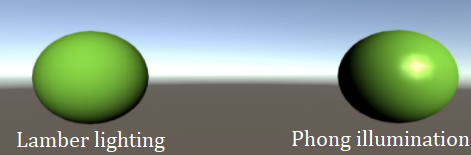
\includegraphics[scale=1.0]{light_pic.png}
    \caption{Calculation methods\cite{schrute}}
    \label{fig:pic}
\end{figure}


\section{Software for lighting in games} \label{fourth}
Calculating and creating lighting for a game is extremely complex, and it would not be possible without software. Simulated illumination is embedded in the 3D modeling software used for game production. Each software product contains algorithms that establish simulated illumination. Every algorithm works on its own principles of how lighting is established or simulated, including shadow appearance and color. \cite{Dynamic-Lighting} They offer a range of light sources and visualize it for various environments and situations. The software also plays a role in rendering the image to make it clear. Light-mapping is also built-in for much 3D modeling software. It calculates the brightness of surfaces in a game. Light-maps are then overlaid on top of scene geometry to create the effect of lighting. This process is supported by graphics acceleration hardware that makes light-maps quite useful in 3D real-time applications.\cite{Fast-Lighting} \cite{Unity}


\subsection{Examples of software} \label{examples}

Since each software works with different algorithms, each one is used for a different purpose. A software that has been popular for a long time is Cinema 4D. It has been used in many famous movies for its ability to create mesmerizing visual effects. Another well-liked software is Maya. It has slightly better tools than Cinema 4D, however, it has a steeper learning curve. In order to discover Maya’s full potential, a certain level of coding ability is required. That means you should understand Python and also Maya’s own Maya Embedded language. \cite{maya} Furthermore, Blender is a free Open source alternative for indie game developers. It offers a wide range of tools for creating a professional-looking computer game. The last software to be mentioned is 3ds Max. It is owned by the same company as Maya, however, it is more famous for its visualization and game design tools. \cite{maya} In terms of lighting, you can save time with centralized creative tools for interactive light mixing, color correction, and lens effects on the rendered image.\cite{3ds} 

Table \ref{table} summarizes facts about popular software that is often used to simulate lighting in computer games. 
\begin{table}[h!]
\begin{center}
 \begin{tabular}{|c||c|c|c|} 
 \hline
 Software & Company & Utilization & Price a year \\ 
 \hline\hline
 Maya & Autodesk & Publisher games & 215\$ \\ 
 \hline
 3ds Max & Autodesk & Industry standard & 215\$ \\
 \hline
 Blender & Open source & Indie computer games & free \\
 \hline
 Cinema 4D & Maxon & Creating movies and games & 719\$ \\
 \hline
\end{tabular}
\end{center}
\caption{Software for lighting in games\cite{software}}
\label{table}
\end{table}

\section{Rendering of lighting} \label{fifth}
The process of rendering is used to portray 3D characters frame by frame on a 2D screen. This article will mention the three most frequently used rendering techniques for computer games.

\paragraph{Rasterization.}
A raster image is composed of a collection of shaded pixels. The GPU will tell the game to create a 3D image out of small shapes, most often triangles. These triangles are turned into individual pixels and then put through a shader to create the image on the screen. This process is often carried out by fixed-function hardware within the graphics pipeline.\cite{wang}
An example of OpenGL graphics pipeline is shown in the figure \ref{fig:diag2}.

\begin{figure}[ht]
    \centering
    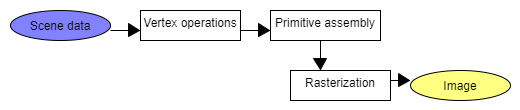
\includegraphics[scale=0.5]{diag_gr.png}
    \caption{OpenGL graphics pipeline\cite{software}}
    \label{fig:diag2}
\end{figure}

\paragraph{Ray tracing.}
Ray tracing simulates how light acts in real the real world. The objects we see are illuminated by various light sources. The photons, which are particles of light, can bounce from one object to another before reaching our eyes. On the way, the light may be blocked in some areas, creating shadows. Moreover, refraction might be created when light passes through a body of water. Ray tracing captures this process with a view camera. It is like an eye that traces the path of a light ray through each pixel on a 2D viewing surface. Then it applies the tracing into a 3D model of the scene. \cite{caulfield}

\paragraph{RTX Global Illumination.}
With the arrival of more powerful GPUs, a new method for ray tracing was created. The company NVIDIA built a ray-tracing technology that makes quality, real-time rendering possible for game developers. It required a decade of work in computer graphics algorithms and GPU architectures. \cite{caulfield}

\subsection{Comparison} \label{comparison}

The diagram in the figure \ref{fig:diag} contains a mind map with the rendering techniques and their most significant attributes. 
 
 \begin{figure}[ht]
    \centering
    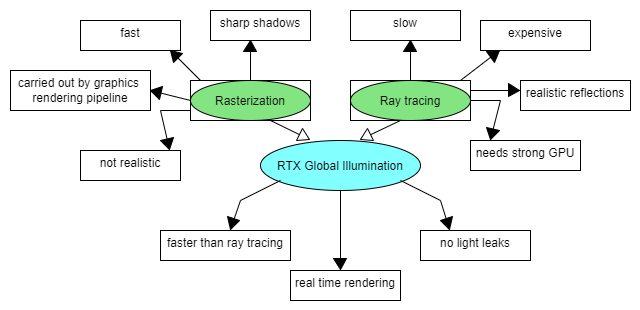
\includegraphics[scale=0.5]{diag.png}
    \caption{Rendering methods\cite{caulfield} \cite{wang}}
    \label{fig:diag}
\end{figure}

Each of these methods has its pros and cons. Since rasterization is extremely fast consequently, it has been a good option for video game graphics for a long time. However, it has its limitation when it comes to colors and shadows. Also, it is not completely realistic. Therefore, the ray-tracing technique should be taken into consideration. Scenes that equip this technique are much more lifelike.\cite{wang} The drawback of this technique is its lack of speed and the need for expensive computation power. This is where the hybrid technique, RTX Global Illumination, which uses elements from both previous techniques comes to play. It is a faster version of ray tracing that uses real-time rendering. Therefore, it can be used for computer games. In a few years, it might become the standard for game developers. It could give the games cinematic qualities of movies.\cite{caulfield} 

\section{Reaction to the themes from the lectures} \label{sixth} 

\paragraph{Social context.}
Computer science is not only about computers. The work of an engineer has a huge social impact. Since we live in the age of software and hardware breakthroughs, numerous work positions have been created thanks to it. Many pieces of research deal with new developments of technologies. In my view, the development of computer games is one of the quickly developing fields. Playing computer games is a part of life for numerous humans. Therefore, even the social influence of software, which makes lighting more believable in computer games, is undeniable.

\paragraph{Historical context.}
The historical context of computer science, which was discussed in lecture 5, was very enriching for me. It was about notable IT personalities, who unfortunately passed away recently. Learning about those IT people, who made a difference in the world, was an inspiring experience. For instance, Russel Kirsch, who invented pixel, is especially important when talking about the topic of lighting in computer games. Pixels are a crucial part of graphics, and therefore without Russel Kirsch, the field of computer graphics could be much different today.

\paragraph{Technology and people.}
This lecture explained how huge projects are realized, even with some imperfections in the specifications. An effective framework, called SCRUM, works in iterations with an increment after each one. The team works in sprints, and each sprint consists of a doable amount of work. It also takes human qualities into account. It is definitely beneficial to use this framework during the development of a computer game. It would not be possible to make a game all at once - iterations are necessary. Many people are participating in the process, and they need to be organized. However, after each sprint, there should be a meeting where they can discuss their progress. That way, people can implement their knowledge in the new iterations.

\paragraph{Sustainability and ethics.}
This lecture made me think about the ethics of the fast development we experience these days. It cannot be stopped, however, it should be sustainable. In my opinion, the waste should be reduced to the minimum, even when creating software. The lecture also mentioned the Software Engineering Code of Ethics. I find the principle that states, software engineers should ensure the highest professional standards of their products crucial.

\section{Conclusion} \label{seventh} 
In conclusion, the significance of lighting in computer games is undeniable. Artistic lighting induces pleasant emotions in the players, and dark shadows can give the game an eerie feeling. There are some basic types of lighting used in computer games. To create a scene, they are sometimes interconnected. Developing software for lighting would not be possible without calculation methods for illumination. Nowadays, there is much software that deals with lighting simulation in computer games. Each one works with an independent algorithm and with various rendering techniques. The rendering techniques had a breakthrough recently, with the NVIDIA RTX Global Illumination. Hopefully, we will see this technology used more in real life soon.

\bibliography{literatura}
\bibliographystyle{plain} 
\end{document}
